
\chapter{Methodology}

\section*{Solution proposal}

We present our proposed solution for the acoustic inspection of metal structures using multi-robot navigation strategies.
We have developed three specific strategies to optimize data acquisition and enable the tomography of metallic surfaces.
These three strategies are:
\begin{enumerate}
	\item \textit{Roller Painting} navigation strategy
	\item \textit{Nordic Skiing} navigation strategy
	\item \textit{Polygonal Investigation} navigation strategy
\end{enumerate}
Among these strategies, the first two are non-reactive and can be considered as coarse exploration strategies, the goal being to quickly obtain a global coverage of the surface to be inspected.
The third strategy is reactive and makes it possible to optimize the acquisition of data for the realization of the tomography.
These three strategies aim to map the metal surface and detect areas of corrosion.
We define these three navigation strategies in the following subsections.
We also explain how the data structure used for mapping corrosion areas, an occupancy grid, is updated based on information collected by the robots' UGW sensors.

\subsection*{Occupancy grid update process for mapping}

When scanning the surface to be inspected by a pair of transmitter and receiver robots, the transmitter robot emits an acoustic wave in the metal structure, which is then received by the receiver robot.
The detection being considered as perfect, the receiver robot receives the wave emitted by the transmitter robot, without quasi-alteration of the power of the signal, if and only if the line segment between the two robots does not cross a zone of corrosion.
It is thus possible to determine whether a corrosion zone is present between the two robots by checking whether the signal received by the receiving robot is sufficiently powerful.
Insofar as there is no detection of corrosion between the transmitter and the receiver, then the line segment between the two robots is considered to be free of corrosion.
Otherwise, then the points of the line segment between the two robots are considered to be corrosion, with the exception of the points previously perceived to be free of corrosion.
The presence of corrosion on the segment is therefore overestimated.
The displacement strategies will aim to carry out several measurements, to reduce this overestimation, and approach the real shape of the corrosion.

We now only need to determine which cells of the occupancy grid are crossed by the line segment between the two robots.
% For this we use Bresenham's segment drawing algorithm~\cite{enwiki:1155124335} which is commonly used to determine the points of a discrete plane that need to be drawn in order to form an approximation of a line segment between two points given.
We detail our implementation of this algorithm in section~\ref{subsec:Bresenham}.

As the metal surface is explored, the occupation grid is updated based on the information gathered by the robots.
More precisely, the cells of the occupancy grid that identify corrosion elements are updated with the occupied state, while the cells that identify healthy areas are updated with the empty state.
We thus end up with an occupation grid which represents the state of corrosion of the metal surface, with, for each corrosion zone, an approximation of the convex envelope of the corrosion zone.

\subsection*{\textit{Roller Painting} navigation strategy}

The first navigation strategy we propose is the \textit{Roller Painting} navigation strategy.
We chose this name for this strategy because the movement of the robots during this strategy is similar to that of a paint roller when painting a wall.
This strategy is based on a rough exploration of the surface to be inspected, where the robots move in a straight line on parallel trajectories, guaranteeing global coverage of the inspection area.
It is therefore a question here of carrying out a grid of the surface to be inspected.

\begin{figure}[h!]
	\centering
	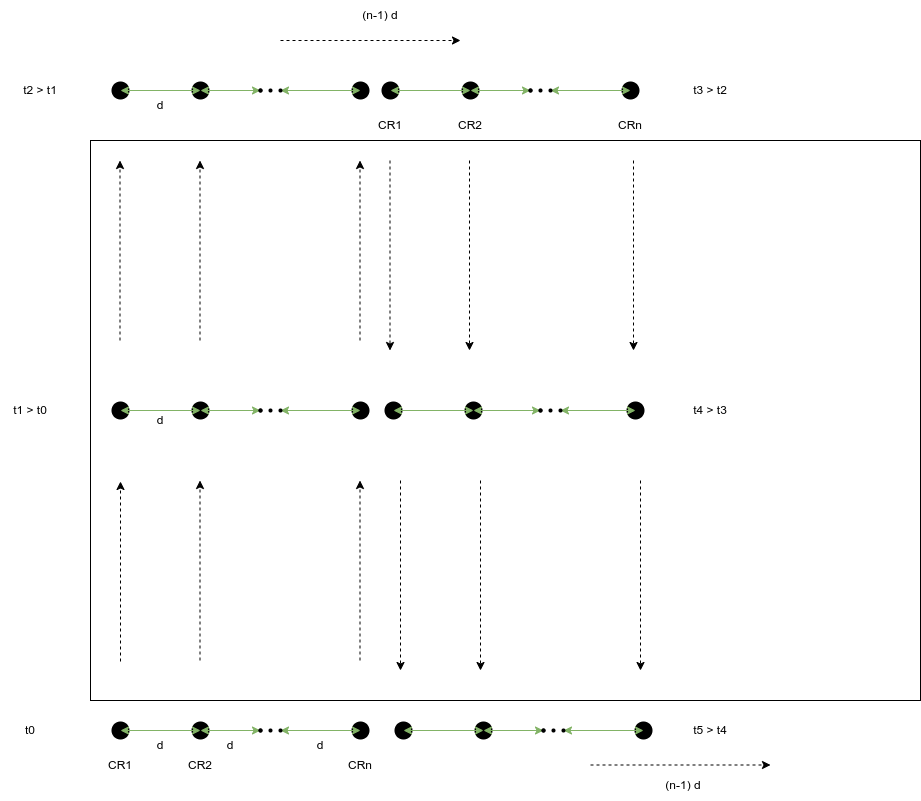
\includegraphics[scale=0.5]{graphics/peinture_au_rouleau.png}
	\caption{\textit{Roller Painting} navigation strategy.}
	\label{fig:peinture_au_rouleau}
\end{figure}

We present in figure~\ref{fig:peinture_au_rouleau} a diagram describing the paint roller navigation strategy.
This strategy consists of two phases, a vertical movement phase and a horizontal movement phase.
The figure~\ref{fig:peinture_au_rouleau} shows the first phase of vertical displacement.
In order to achieve this strategy, a minimum of, $n \ge 2$ robots, aligned horizontally and separated by a distance $d < d_{max}$, is used.
These robots move vertically, simultaneously, following a parallel trajectory.
Once the end of the surface to be inspected has been reached, the robots rotate 90 degrees and move horizontally, simultaneously, by a distance $(n - 1) \cdot d$.
They then perform a new 90 degree rotation and move again vertically, in a straight line, simultaneously, following a path parallel to each other, until they reach the other end of the surface to be inspected.
This process is repeated until the metal surface is fully inspected.
The same process is then repeated, but this time horizontally.

During this strategy, each robot is both a transmitter and a receiver of UGW waves.
If the distance separating a robot $n_a$ from a robot $n_b$, $(n_a, n_b) \in \{1, 2, \dots, n\}^2$, is less than the maximum propagation distance UGW waves, $d_{max}$, then the robot $n_a$ is able to receive the signal emitted by the robot $n_b$ and vice versa.
However, it is not necessary for a robot $n_k$, $n_k \in \{1, 2, \dots, n\}$, to process signals received from all other robots.
Indeed, the robots being aligned, the signals received from the robots $n_{k-1}$ and $n_{k+1}$, are sufficient for the reconstruction of the state of the metallic surface.
The waves emitted by the robots $n_1, n_2, \dots, n_{k-2}$ and $n_{k+2}, \dots, n_n$ are not useful for the robot $n_k$.
The robot $n_k$ can therefore ignore these signals and concentrate only on the signals received from the robots $n_{k-1}$ and $n_{k+1}$.
Insofar as the first signals perceived by the robot $n_k$ are those emitted by the robots $n_{k-1}$ and $n_{k+1}$, due to their proximity, it is possible for the robot $n_k$ to filter signals received from other robots.
This constitutes an optimization in terms of processing for each robot.

The fact that the robots move along a parallel trajectory and simultaneously, implies that the rays of the signal emitted by the transmitter robot and received by the receiver robot, always have an orientation of $0$ radian for the vertical phase and an orientation of $\frac{\pi}{2}$ radians for the horizontal phase.
There is therefore not a large variation in the orientation of the transmitted and received signal.
Thus, this strategy will only be able to approach the convex hulls of the corrosion zones by rectangles.
Examples of occupancy grids resulting from the \textit{Roller Painting} navigation strategy, represented as images, where the cells of the grid correspond to the pixels of the images, are shown in appendix~\ref{annexe:resultat}, figure~\ref{fig:peinture_au_rouleau_resultats}.

\subsection*{\textit{Nordic Skiing} navigation strategy}

The second strategy we propose is the navigation strategy \textit{Nordic skiing}.
We chose this name for this strategy because the movement of the robots during this strategy is similar to the movement of a skier's skis.
This strategy still consists of moving in a straight line and following parallel trajectories, but this time the robots move sequentially and no longer simultaneously.
In this strategy, we wanted to increase the orientation diversity of the transmitted and received signal rays, in order to approach more precisely the convex hulls of the corrosion zones.

\begin{figure}[h!]
	\centering
	\begin{subfigure}[t]{0.45\linewidth}
		\centering
		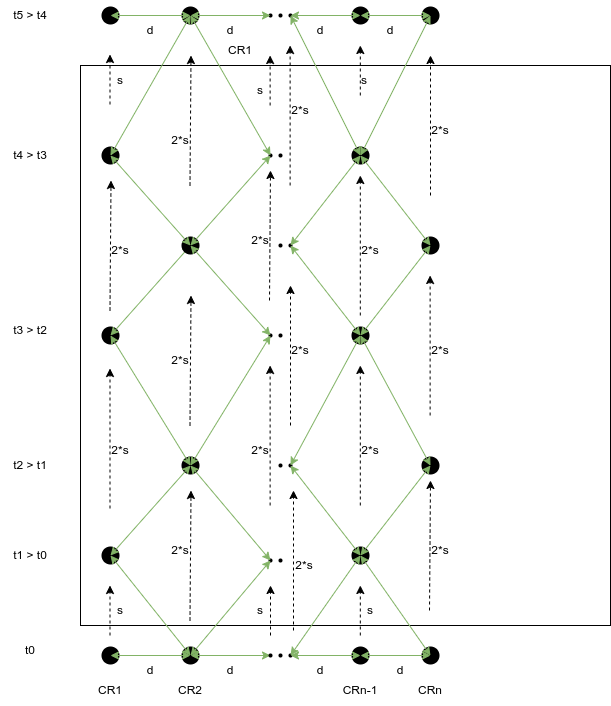
\includegraphics[width=\linewidth]{graphics/ski_nordique_1.png}
		\caption{\textit{Nordic Skiing} navigation strategy - first phase.}
		\label{fig:ski_nordique_1}
	\end{subfigure}
	\hfill
	\begin{subfigure}[t]{0.45\linewidth}
		\centering
		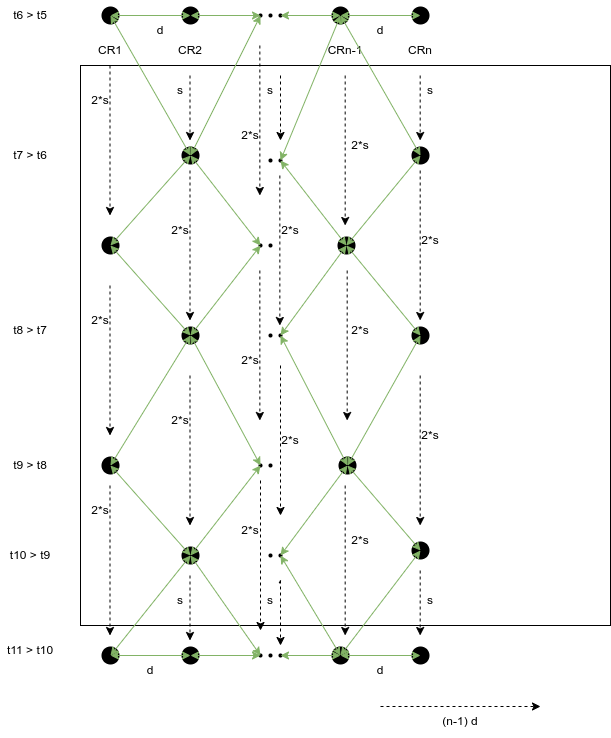
\includegraphics[width=\linewidth]{graphics/ski_nordique_2.png}
		\caption{\textit{Nordic Skiing} navigation strategy - second phase.}
		\label{fig:ski_nordique_2}
	\end{subfigure}
	\caption{\textit{Nordic Skiing} navigation strategy.}
	\label{fig:ski_nordique}
\end{figure}

Figure~\ref{fig:ski_nordique} presents a diagram describing the navigation strategy \textit{Nordic Skiing}.
This strategy also consists of two phases, a vertical movement phase and a horizontal movement phase.
Figure~\ref{fig:ski_nordique} shows the first phase of vertical movement.
In order to achieve this strategy, a minimum of, $n \ge 2$ robots, aligned horizontally and separated by a distance $d < d_{max}$, is used.
These robots move vertically, following a parallel path, but sequentially.
The odd robots move in a straight line a distance $s$ and stop.
The even robots then move in a straight line a distance of $2 \cdot s$ and stop.
This process is repeated until the end of the surface is reached (figure \ref{fig:ski_nordique_1}).
Then, the robots repeat this same process, in the opposite direction and so that the stopping points of the robots are not the same as those previously (figure \ref{fig:ski_nordique_2}).
That is to say that this time, it is the even robots which start by moving in a straight line for a distance $s$ and then stop.
Then the odd robots move in a straight line for a distance of $2 \cdot s$ and then stop.
The robots then move horizontally a distance $(n - 1) \cdot d$ and repeat the same process until the metal surface is fully inspected.
The same process is then repeated, but this time horizontally.
In order for the various receiver robots to be able to receive the signals emitted by the transmitter robots, it is also necessary to impose that $s$ be strictly less than $\frac{d_{max}}{2}$, i.e. $s < \frac{d_ {max}}{2}$.

During this strategy, each robot is both a transmitter and a receiver of UGW waves.
Here, as with the \textit{Roller Painting} navigation strategy, it is not necessary for a robot $n_k$, $n_k \in \{1, 2, \dots, n\}$, to process the signals received by robots other than $n_{k-1}$ and $n_{k+1}$.

The fact that the robots move following a parallel trajectory, but in a sequential way, implies that the rays of the signal emitted by the transmitter robot and received by the receiver robot, have an orientation of greater variation.
Thus, this strategy makes it possible to approximate the convex envelopes of the corrosion zones by more diverse and precise shapes than rectangles.
Examples of occupation grids resulting from the navigation strategy \textit{Nordic Skiing}, represented in the form of images, where the cells of the grid correspond to the pixels of the images, are shown in appendix~\ref{annexe:resultat}, figure~\ref{fig:ski_nordique_resultats} and figure~\ref{fig:ski_nordique_resultats_2}.

\subsection*{\textit{Polygonal Investigation} navigation strategy}

The third strategy we propose is the \textit{Polygonal Investigation} navigation strategy.
We have seen, previously, that at the end of the realization of the navigation strategy \textit{Roller Painting}, the convex hull of the corrosion zones was approximated by a rectangle.
This approximation is a little more precise for the navigation strategy \textit{Nordic Skiing}.
It would be interesting to have a greater degree of precision around potential areas of corrosion.
This is what we propose with the navigation strategy \textit{Polygonal Investigation}.
This strategy consists of investigating around potential areas of corrosion, previously detected by one of the two previous navigation strategies.
It consists of positioning the robots around the corrosion zones and making them move along a polygonal trajectory, so that the rays of the signal emitted and received have an orientation of greater variation even around these zones.

\begin{figure}[h!]
	\centering
	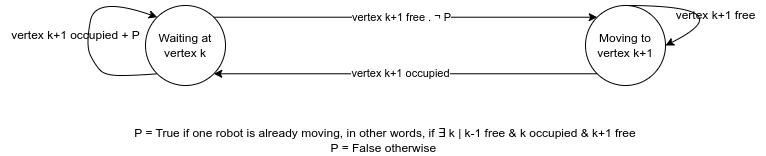
\includegraphics[scale=0.6]{graphics/automat_poly.png}
	\caption{\textit{Polygonal Investigation} navigation strategy.}
	\label{fig:automat}
\end{figure}

We present in figure~\ref{fig:automat} a finite state automaton describing the navigation strategy \textit{Polygonal Investigation}.
At the beginning of the \textit{Polygonal Investigation} navigation strategy, each $n \in \mathbb{N}$ robots of $k \in \mathbb{N}$ teams are positioned on consecutive vertices of a polygon enclosing the potential area of corrosion.
In the latter, each robot has two states.
The first consists of waiting and the second consists of moving along the polygonal trajectory, namely traversing the various vertices that make up the polygon.
The robot capable of advancing, that is to say, whose next vertex is not occupied by another robot, advances.
The others wait until the advancing robot reaches the last free vertex of the polygon.
The process is then repeated for each robot of each team until the vertices occupied by the robots are the same as those occupied at the beginning of the navigation strategy \textit{Polygonal Investigation}.

\begin{figure}[h!]
	\centering
	\begin{subfigure}[t]{0.3\linewidth}
		\centering
		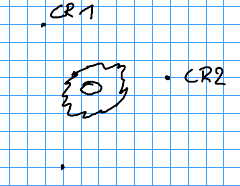
\includegraphics[width=\linewidth]{graphics/triangle_1.png}
		\caption{Initial phase.}
		\label{fig:triangle_1}
	\end{subfigure}
	\hfill
	\begin{subfigure}[t]{0.3\linewidth}
		\centering
		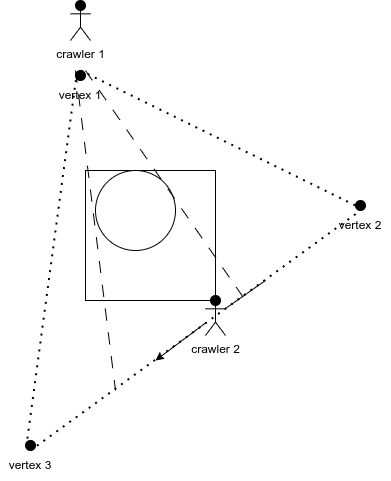
\includegraphics[width=\linewidth]{graphics/triangle_2.png}
		\caption{First phase of movement.}
		\label{fig:triangle_2}
	\end{subfigure}
	\hfill
	\begin{subfigure}[t]{0.3\linewidth}
		\centering
		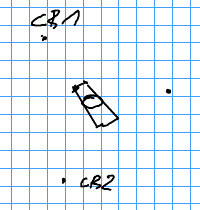
\includegraphics[width=\linewidth]{graphics/triangle_3.png}
		\caption{Second phase.}
		\label{fig:triangle_3}
	\end{subfigure}
	\hfill
	\begin{subfigure}[t]{0.3\linewidth}
		\centering
		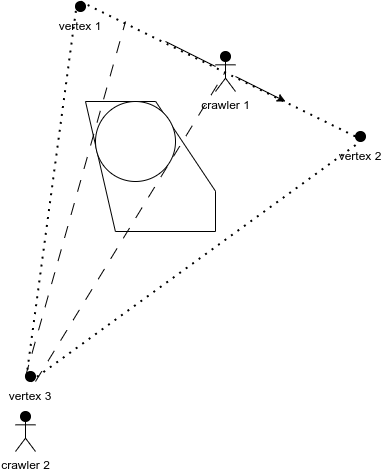
\includegraphics[width=\linewidth]{graphics/triangle_4.png}
		\caption{Second phase of movement.}
		\label{fig:triangle_4}
	\end{subfigure}
	\hfill
	\begin{subfigure}[t]{0.3\linewidth}
		\centering
		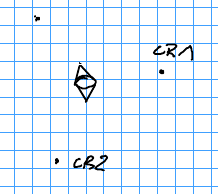
\includegraphics[width=\linewidth]{graphics/triangle_5.png}
		\caption{Third phase.}
		\label{fig:triangle_5}
	\end{subfigure}
	\hfill
	\begin{subfigure}[t]{0.3\linewidth}
		\centering
		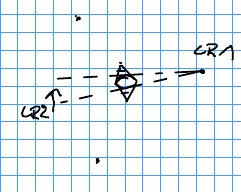
\includegraphics[width=\linewidth]{graphics/triangle_6.png}
		\caption{Third phase of movement..}
		\label{fig:triangle_6}
	\end{subfigure}
	\hfill
	\begin{subfigure}[t]{0.3\linewidth}
		\centering
		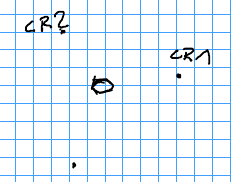
\includegraphics[width=\linewidth]{graphics/triangle_7.png}
		\caption{Last phase.}
		\label{fig:triangle_7}
	\end{subfigure}
		\caption{Movement phases of the \textit{Polygonal Investigation} navigation strategy.}
		\label{fig:triangle}
\end{figure}

We present in figure~\ref{fig:triangle} an example of the different moving phases of the navigation strategy, \textit{Polygonal Investigation} with $k = 1$ team, $n = 2$ robots and a polygon with 3 peaks.
On these different figures, we have represented a corrosion zone by a circle and an approximation of this zone by a shape enveloping the circle.
The objective is to approach the corrosion zone as finely as possible.
The corrosion zone is not known in advance, only the shape enveloping the circle is known.
Figure~\ref{fig:triangle_1} presents the initial phase of the navigation strategy \textit{polygonal investigation}.
Figure~\ref{fig:triangle_2} shows the first moving phase of the \textit{Polygonal Investigation} navigation strategy, while the crawler $CR2$ moves forward.
We can see that after the $CR2$ crawler has moved forward, part of the suspected corrosion area is removed and considered healthy, as we can see in fig~\ref{fig:triangle_3}.
The crawlers keep moving until they reach their initial position, as we can see in figure~\ref{fig:triangle_7}.

\begin{definition}[Phantom zone]
	\label{def:fantomas}
	A phantom zone is a corrosion zone detected by one of the navigation strategies, but which is not a corrosion zone. It is a false positive.
\end{definition}

The \textit{Polygonal Investigation} navigation strategy has two advantages.
The first is that it quickly eliminates phantom zones~\ref{def:fantomas}.
The second is that it makes it possible to approach the convex envelopes of the corrosion zones by more diverse and precise shapes than rectangles due to the great variation in the orientation of the rays of the signal emitted and received by the robots around each vertex of the polygon.

This strategy requires two steps prior to its execution:
\begin{enumerate}
	\item the extraction of the corrosion zones detected by one of the preceding navigation strategies.
	\item determining the order of investigation of corrosion areas.
\end{enumerate}

The first step can be solved using a strongly connected component graph decomposition algorithm.
A strongly connected component is defined at definition~\ref{def:scc}.
We then consider our occupation grid, resulting from the exploration of one of the two previously defined strategies, as an undirected graph $G = (V, E)$, where $V$ is the set of vertices of the graph, corresponding to the cells of the occupancy grid and $E$ are the edges of the graph, corresponds to the adjacent cells.
% This problem is well known and there are simple algorithms to solve it, such as Tarjan's algorithm~\cite{enwiki:1148118528}, of linear time complexity $O(|V| + |E|)$.
We will not look further into this problem and entrust its resolution to the \textit{OpenCV} library.

\begin{definition}[Strongly connected component (SCC)]
	\label{def:scc}
	A strongly connected component of a graph $G = (V, E)$ is a subset $C$ of $V$ such that for any pair of vertices $(u, v) \in C^2$, it there is a path from $u$ to $v$ and a path from $v$ to $u$.
\end{definition}

\begin{definition}[Hamiltonian cycle]
	\label{def:hamilton}
	A Hamiltonian cycle is a cycle passing through all the vertices of a graph, once and only once.
\end{definition}

\begin{definition}[Travelling Salesman Problem (TSP)]
	\label{def:tsp}
	Given a graph $G = (V, E)$, where $V$ is the set of vertices of the graph and $E$ is the set of edges of the graph, and a cost function $c : E \rightarrow \mathbb{R}$, the Traveling Salesman's Problem consists in finding a Hamiltonian cycle~\ref{def:hamilton} of minimal cost in $G$.
\end{definition}

\begin{definition}[Multi-depot multiple Traveling Salesman Problem (mTSP)]
	\label{def:mtsp}
	Given a graph $G = (V, E)$, where $V$ is the set of vertices of the graph and $E$ is the set of edges of the graph, a cost function $c : E \rightarrow \ mathbb{R}$, and a set of depots $D \subset V$, the multi-depot multiple Traveling Salesman Problem is to find a set of cycles of minimum total cost in $G$, each going through one and one single deposit.
\end{definition}

The second step can be solved using a TSP~\ref{def:tsp} (\textit{Travelling Salesman Problem}) algorithm in the case where the number of teams $k$ is equal to 1 and a mTSP ~\ref{def:mtsp} (\textit{(multiple depot) multiple Traveling Salesman Problem}) algorithm in the case where the number of teams $k$ is strictly greater than 1.
There are several solution paradigms to solve this type of problem.
A first is to find an exact solution using an integer linear programming algorithm.
A second is to find an approximate solution using a meta-heuristic.

\begin{definition}[NP Class]
	\label{def:np}
	The class NP is the class of decision problems that can be solved by a non-deterministic algorithm in polynomial time.
\end{definition}

\begin{definition}[NP-hard problem]
	\label{def:nph}
	A problem is NP-hard if it is at least as hard as problems of class NP.
	In other words, a problem is NP-hard if there is a polynomial reduction algorithm that transforms a problem of class NP into an instance of this problem.
\end{definition}

\begin{definition}[NP-complete problem]
	\label{def:npc}
	A problem is NP-complete if it is both NP and NP-hard.
\end{definition}

The traveling salesman problem is an NP-complete~\ref{def:npc} problem.
% It can be treated as an integer linear optimization problem~\cite{article244, gurobi25}.
To do this, we use the formulation presented in equation~\ref{eq:tsp}.

\begin{equation}
	\label{eq:tsp}
	\begin{array}{ll@{}rr}
		\text{minimiser} &
		\displaystyle\sum\limits_{i \in V} \sum\limits_{j \in V} c_{ij} x_{ij} &
		&
		\\
		\text{soumis à} &
		\displaystyle\sum\limits_{i \in V} x_{ij} = 1 &
		&
		\forall j \in V \\
		&
		\displaystyle\sum\limits_{j \in V} x_{ij} = 1 &
		&
		\forall i \in V \\
		&
		\displaystyle\sum\limits_{i \in S} \sum\limits_{j \in S} x_{ij} \leq |S| - 1 &
		&
		\forall S \subset V, 2 \leq |S| \leq |V| - 1 \\
		&
		x_{ij} \in \{0, 1\} &
		&
		\forall i \in V, \forall j \in V \\
	\end{array}
\end{equation}

The objective function to be minimized from the formulation~\ref{eq:tsp} is the sum of the distances between each pair of cities.
The first two constraints ensure that each city is visited exactly once.
The third constraint ensures that the cycle formed by the cities visited is simple, that is to say, that it does not contain sub-cycles.
The last constraint ensures that the decision variables $x_{ij}$ are binary, with $x_{ij} = 1$ if the robot moves from city $i$ to city $j$ and $x_{ij} = 0$ otherwise.

% The mTSP is an NP-hard problem~\ref{def:nph}~\cite{SUNDAR201639}.
% This one can be solved using meta-heuristics like a genetic algorithm~\cite{SinghMTSP, Kiraly2011}

In the next sections, we will detail each navigation strategy, exposing the specific algorithms and mechanisms used to implement our proposed solution. We will also analyze the performance and results obtained through extensive experimentation and evaluation.







\section*{Experiments}

In this section, we present the experiments we conducted to validate and evaluate our different multi-robot navigation and control strategies in the context of acoustic inspection of metal structures.
These experiments aim to demonstrate the efficiency, precision and reliability of our system in detecting and locating corrosion zones.

To carry out these steps, we chose to perform our experiments using \textit{Gazebo}, a well-established simulation environment in the field of robotics.
We started by building several test maps.
These maps model a flat surface on which are placed simple geometric shapes, rectangles and circles, and more complex shapes, polygons between 3 and 8 vertices.
These different geometric shapes represent the corrosion areas that we want to detect and locate.
We present in appendix~\ref{annexe:cartes}, in figure~\ref{fig:test_models} the maps we built for our experiments.
Each of these cards is sized 6 meters by 6 meters.
The number of corrosion zones varies between 5, 8, 11, 15, 20 and 30 zones.
The size and location of corrosion areas are randomly generated.
For the maps of 5, 8, 11 and 15 zones, we generated 5 different maps in order to have more representative results.
We did not allow ourselves to generate several maps for the 20 and 30 zone maps, the polygonal investigation time being too long.

We also simulated the UGW sensor by exploiting the simulation of a UWB sensor.
This UWB sensor makes it possible to emit a pulse and to receive it.
By measuring the signal strength, we are able to know whether the signal has passed through an object or not.
The behavior of this UWB sensor is therefore similar to that of the UGW sensor, namely that it makes it possible to detect the presence of an object between two points, but not to locate it.

We evaluated the performance of the three navigation strategies in terms of Cohen's $\kappa$ and inspection time.
For the \textit{Roller Painting} and \textit{Nordic Skiing} strategy, we only used two robots.
For these two strategies, we varied the distance $d$ between the robots.
For the \textit{Nordic Skiing} strategy, we also varied the pitch $s$ between the robots.
For the \textit{Polygonal Investigation} strategy, we vary the number of robots $n$, the number of teams $k$ and the number of sides $p$ of the polygons used.
We use the result of the navigation strategy \textit{Roller Painting} as a starting point.
We justify this choice by the fact that this strategy is the fastest and least accurate and therefore the most likely to benefit from an improvement from the \textit{Polygonal Investigation} strategy, without reaching inspection times too long.
We therefore vary the parameter $d$ of this strategy.
We summarize the experimental parameters used for each strategy in table~\ref{tab:exp_params}.

\begin{table}[h!]
	\centering
	\begin{tabular}{|c|c|c|}
		\hline
		Strategy & Parameter & Values \\
		\hline
		\multirow{2}{*}{\textit{Roller Painting}} & $n$ & 2 \\
		& $d$ & 1, 2, 3, 6 (meters) \\
		\hline
		\multirow{3}{*}{\textit{Nordic Skiing}} & $n$ & 2 \\
		& $d$ & 1, 2, 3, 6 (meters) \\
		& $s$ & 1, 2, 3, 6 (meters) \\
		\hline
		\multirow{5}{*}{\textit{Polygon Investigation}} & initial strategy & \textit{Roller Painting} \\
		& $d$ & 1, 2, 3, 6 (meters) \\
		& $n$ & 2, 4 \\
		& $k$ & 1, 2 \\
		& $p$ & 4, 6 \\
		\hline
	\end{tabular}
	\caption{Experimental settings used for each navigation strategy.}
	\label{tab:exp_params}
\end{table}

During these simulations, we expect to have certain results.
Among them, we expect the \textit{Roller Painting} strategy to be the fastest, but also the least accurate.
Conversely, we expect the \textit{Polygonal Investigation} strategy to be the most accurate, but also the slowest.
We also expect the $d$ parameter to have an impact on the accuracy and inspection time of the \textit{Roller Painting} and \textit{Nordic Skiing} strategies.
A low $d$ distance should provide better accuracy, but should also increase inspection time.
Moreover, we expect that the $s$ parameter will also have an impact on the accuracy and inspection time of the \textit{Nordic Skiing} strategy.
A low $s$ distance should provide better accuracy, but should also increase inspection time.
We also expect the $p$ parameter to have an impact on the accuracy and inspection time of the \textit{Polygonal Investigation} strategy.
A low number of sides $p$ should provide better accuracy, but should also increase inspection time.
Next, we expect the parameters $k$ and $n$ to have an impact on the inspection time of the \textit{Polygonal Investigation} strategy.
A high number of teams $k$ or a high number of robots $n$ should allow to obtain a lower inspection time.
Finally, we expect the number of corrosion zones to have an impact on the inspection time of the \textit{Polygonal Investigation} strategy, but not on the \textit{Roller Painting} and \textit{Nordic Skiing} strategies.
The higher the number of corrosion areas, the higher the inspection time should be for the \textit{Polygonal Investigation} strategy.
Finally, we expect the number of corrosion zones to have an impact on the accuracy of the different strategies.
The greater the number of corrosion areas, the lower the accuracy should be.
Indeed, the higher the number of corrosion zones, the higher the probability of ghost zones appearing for the \textit{Roller Painting} and \textit{Nordic Skiing} strategies.
For the \textit{Polygonal Investigation} strategy, the higher the number of corrosion zones, the greater the probability that two distinct corrosion zones were confused into one during the \textit{Roller Painting} or \textit{Nordic Skiing} strategies.

% \begin{table}[h!]
% 	\centering
% 	\begin{tabular}{|c|c|c|c|}
% 		\hline
% 		Strategy & Parameters & Score & Time \\
% 		\hline
% 		\multirow{5}{*}{\textit{Roller Painting}} & medium density, $d$ medium & - & ++ \\
% 		\cline{2-4}
% 		& low density & + & ++ \\
% 		& high density & - - & ++ \\
% 		& low $d$ & + & + \\
% 		& strong $d$ & - - & +++ \\
% 		\hline
% 		\multirow{7}{*}{\textit{Nordic Skiing}} & medium density, $d$ medium, $s$ medium & ++ & - \\
% 		\cline{2-4}
% 		& low density & +++ & - \\
% 		& high density & + & - \\
% 		& low $d$ & +++ & - - \\
% 		& strong $d$ & + & + \\
% 		& low $s$ & +++ & - - \\
% 		& strong $s$ & + & + \\
% 		\hline
% 		\multirow{9}{*}{\textit{Polygonal Investigation}} & mean density, mean $n$, mean $k$, mean $p$ & +++ & - \\
% 		\cline{2-4}
% 		& low density & ++++ & + \\
% 		& high density & ++ & - - \\
% 		& low $n$ & +++ & - - \\
% 		& strong $n$ & +++ & + \\
% 		& low $k$ & +++ & - - \\
% 		& loud $k$ & +++ & + \\
% 		& low $p$ & ++ & + \\
% 		& strong $p$ & ++++ & - - \\
% 		\hline
% 	\end{tabular}
% 	\caption{Expected results for each navigation strategy.}
% 	\label{tab:expected_results}
% \end{table}

% For the sake of clarity, we summarize in table~\ref{tab:expected_results} the expected results for each navigation strategy.
% The table presents the expected results for each navigation strategy, according to the different experimental parameters.
% Navigation strategies include \textit{Roller Painting}, \textit{Nordic Skiing}, and \textit{Polygonal Investigation}.
% Parameters include density, distance $d$, pitch $s$, number of sides of a polygon used in polygonal investigation $p$, number of teams $k$ and number of robots $ n$.

% For each strategy, the table indicates the expected scores and times associated with each of the parameters compared to the expected scores and times for the intermediate parameters.
% The scores are represented by "+" and "-" symbols and indicate the expected level of precision.
% The times are also indicated by "+" and "-" symbols and reflect the expected inspection slowness.
% Thus a ++ score is considered more accurate than a + score, and a - - time is considered slower than a - time, for example.

The different results from the different simulations carried out are available in appendix~\ref{annexe:resultat}.
On these images, it is possible to see in black the real areas of corrosion and in blue the areas detected as having corrosion by the various navigation algorithms.

